\chapter{Background}

The foundational principle of neural networks is, in its purest form, inspired by the biology of the human brain.
The field of AI has often modelled new algorithms after biological phenomena; in this field, genetic algorithms are based on evolution and particle swarm optimization is based on social behaviors.


LeCun et al's seminal work in this field, \emph{Gradient-Based Learning Applied to Document Recognition} \cite{lecun1998gradient}, provided the first basis of using backpropagation methodologies to train visual classifiers.
Even more importantly, it introduced the fundamental structure of the modern visual deep learning network.
In its usage of convolutions as a method for extracting high-level features out of larger images, it set the framework for a new style of network that would prove to be far more efficient and scalable.

A convolution is a operator applied to two functions $f$ and $g$, which provides a way of interpreting one function in the context of the other.
The operation is generally defined as
\[(f * g)(t) = \int_{-\infty}^\infty f(r)g(t-r) dr\]
In the perspective of modern deep learning, we are primarily interested in its usage as a matrix operator; in this context, we limit the range of $g$ to the size of the matrix $s$ such that
\[(f * g)(t) = \int_0^s f(r)g(t-r) dr\]
In this context, we refer to $g$ as the \emph{convolutional kernel}.
Using a convolutional kernel to preprocess the image proves to be a critical to the performance of modern deep learning methods, as a small kernel can operate over a large image in parallel.
Figure~\ref{fig:gimp_edge} shows a simple convolutional kernel can produce high-level details of an image.
In this example, we consider the basic edge-detecting matrix 
\[E = \begin{bmatrix} 0 & 1 & 0 \\ 1 & -4 & 1 \\ 0 & 1 & 0\end{bmatrix}\]


\begin{figure}[!htb]
    \begin{subfigure}{0.5\textwidth}
    \centering
    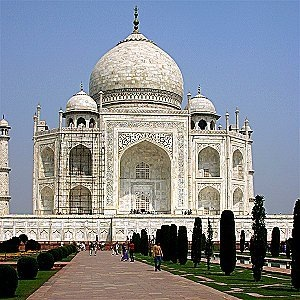
\includegraphics{images/gimp_original}
    \end{subfigure}%
    %
    \begin{subfigure}{0.5\textwidth}
    \centering
    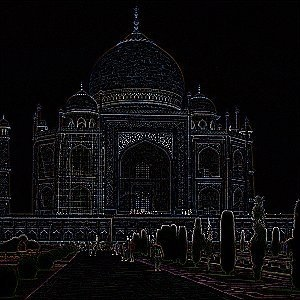
\includegraphics{images/gimp_edgedetect}
    \end{subfigure}

\caption{A demonstration of an edge-detecting convolution, from the GIMP User's Manual. \cite{gimpconvolution}}
\label{fig:gimp_edge}
\end{figure}

Convolutional neural networks are therefore the product of using these 

% overparametrization


